\section{Design}\label{kapitel5}
%sign(rund und Böbbel), Gamification, Datenflüsse?
%Einschränkungen bei der Länge der Läufe
\subsection{Datenbank}
\begin{figure}[!h]
\centering
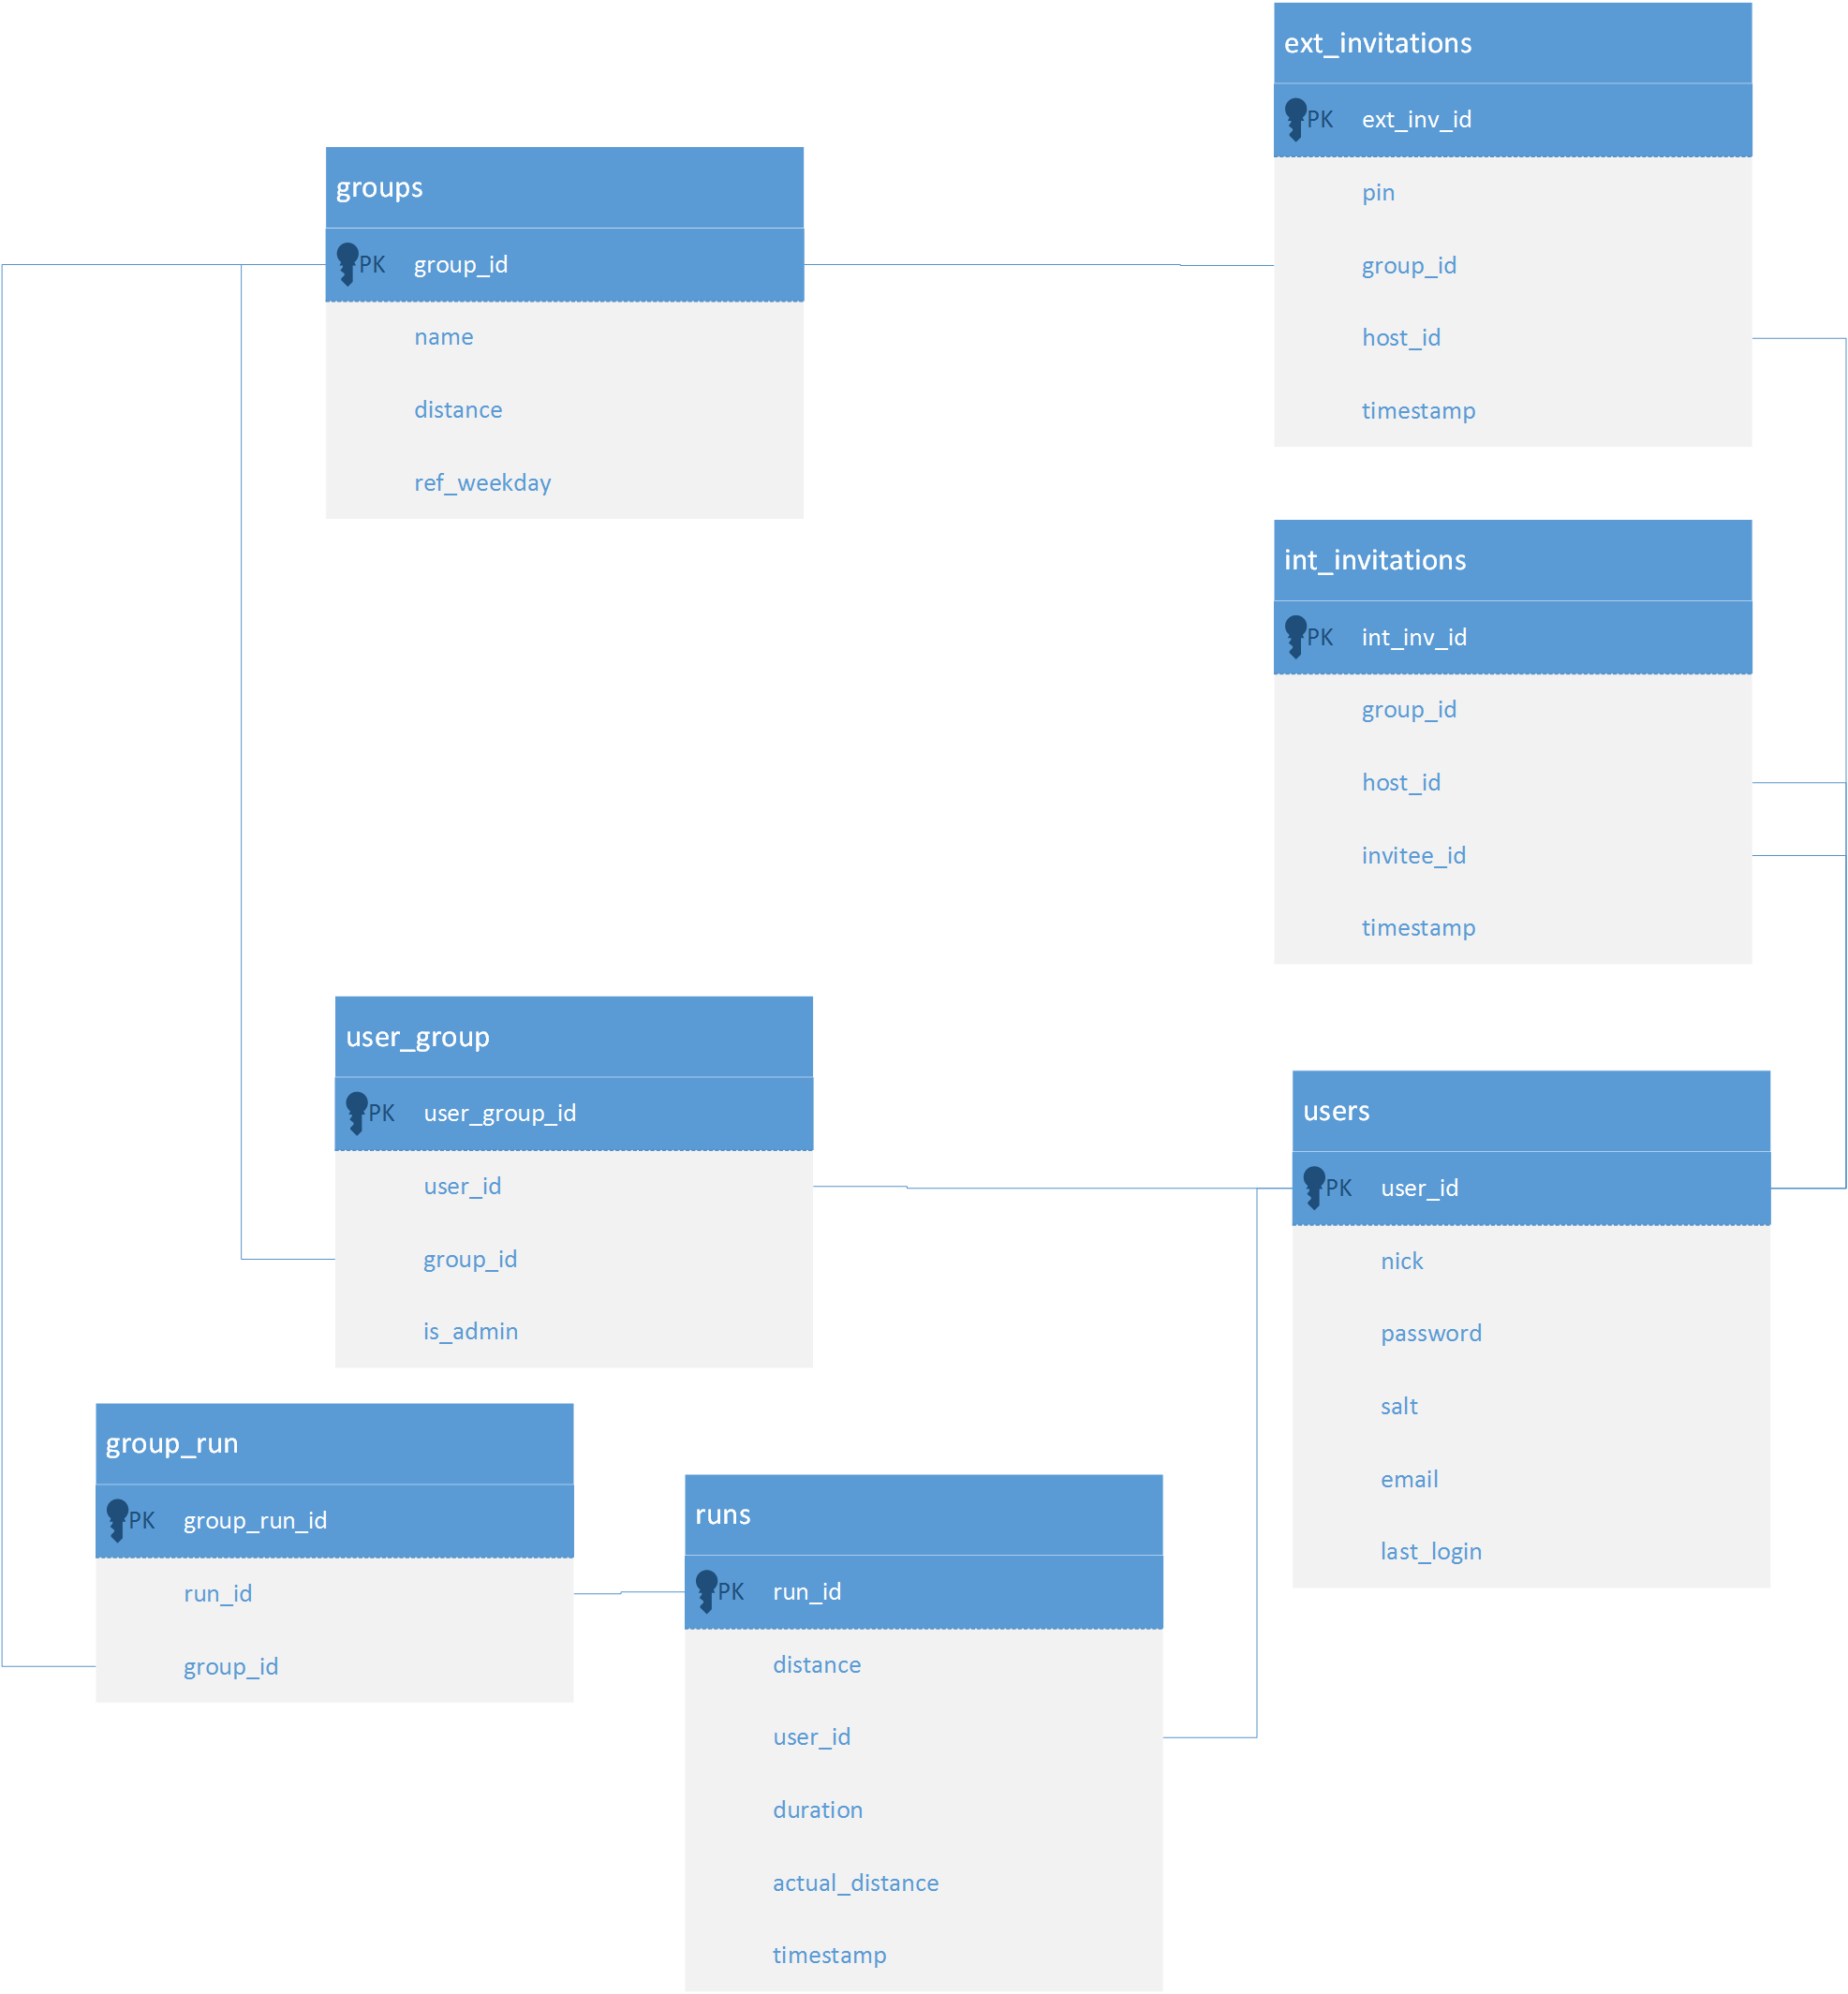
\includegraphics[width=\textwidth]{abb/er_diagram}
\caption{Datenbankschema}
\end{figure}
Die Datenbank besteht aus Tabellen für den Nutzer, die Gruppen, internen als auch externen Einladungen und den Läufen. Zusätzlich bestehen zwei weitere Tabellen für das Abbilden von n:m-Beziehungen.

Jeder Tabelle ist ein Primärschlüssel zuegordnet um eine eindeutige Identifikation jedes Tupels zu ermöglichen.

Jedem Nutzer ist ein einzigartiger Nutzername, ein verschlüsseltes Passwort, ein Salt für die Hashingfunktion, eine E-Mail-Adresse und ein Zeitstempel des letzten Logins zugeordnet.

Eine Gruppe besteht aus dem Namen, der vorgegebenen Laufdistanz und einem wöchtentlichen Stichtag, zu dem die Läufe der davorliegenden Woche ausgewertet werden. Dieser besteht aus einer Ganzkommazahl zwischen null und sechs, welche die Wochentage beginnend mit Sonntag enumeriert.

Es kann eine unbegrenzte Anzahl an Nutzern einer Gruppe beitreten und Nutzer können beliebig vielen Gruppen beitreten. Es handelt sich also um eine n:m-Relation, die anhand der Tabelle user\_group dargestellt ist. Zusätzlich wird in user\_group festgehalten, ob es sich bei dem Nutzer um einen Gruppenadministratoren handelt. Hier steht die ``1'' für ``Admin'' und die ``0'' für ``Nichtadmin''.

Eine weitere n:m-Relation mittels der Tabelle group\_run zwischen Läufen und Gruppen. Dem Lauf sind die Attribute Distanz, Nutzer-ID, Dauer, die wirkliche Distanz und ein Zeitstempel zugeordnet. Die Nutzer-ID stellt eine 1:1-Beziehung auf den Nutzer dar.

Des weiteren wurden die Tabellen ext\_invitations und int\_invitations angelegt.

Externe Einladungen sind Einladungen an Andere außerhalb der App. Es wird eine PIN geteilt, mit dem der Eingeladene später die Einladung annehmen kann. Diese ist eine 10-stellige Ganzkommazahl, Außerdem befinden sich in der Tabelle die Gruppen-ID und die Nutzer-ID, welche jeweils 1:1-Beziehungen markieren sowie ein Zeitstempel.

Interne Einladungen gehen an andere Nutzer der App. Hier sind die Attribute die ID des Einladenden, des Eingeladenen und der Gruppe. Außerdem besteht auch hier ein Zeitstempel.
%TODO Logout-->Login/Register, Kick User ist keine eigene Seite, kick nur wenn admin
\subsection{Navigationsschema}
\begin{figure}[htb]
\centering
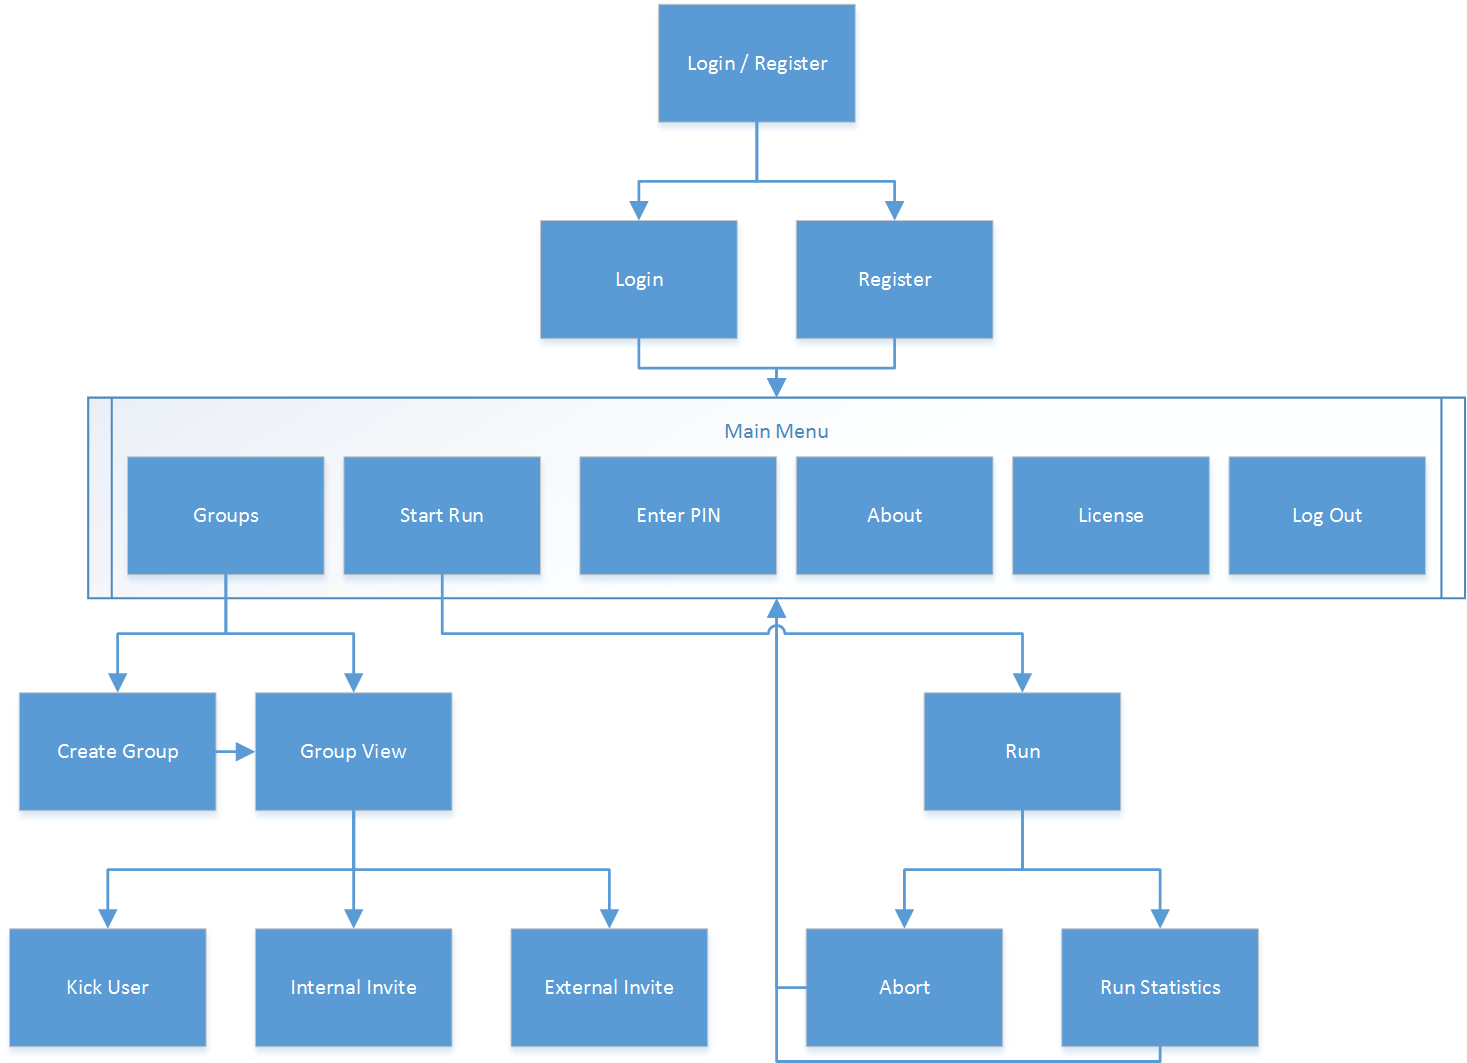
\includegraphics[width=\textwidth]{abb/navigation_diagram}
\caption{Navigationsdiagramm}
\end{figure}

%Warum was wo und wie
Nach dem Anmelden bzw. Registrieren befindet sich der Nutzer in der Gruppenübersicht. Diese ist Teil des Navigationsmenüs. Aus diesem lassen sich alle wichtigen Funktionalitäten erreichen:
\begin{itemize}
\item Gruppenübersicht - Auflistung der eigenen Gruppen und der Einladungen in Gruppen
\item Laufen - Erster Schritt zum Start des Laufs. Es wird dem Nutzer die Wahl gegeben für welche Gruppen er laufen möchte bzw. auf welcher Distanz.
\item PIN-Eingabe - Eingabe der PIN, die der Nutzer bei einer externen Einladung erhält.
\item Über - Hier stehen kurze Informationen über das Team.
\item Lizenz - Hier befindet sich die Lizenz unter der die App steht; die GNU Public License. 
\item Abmelden - Hier kann sich der Nutzer abmelden, um zurück zur Anmeldung / Registrierung zu gelangen.
\end{itemize}

Das Hauptmenü ist ein seitliches Menü, welches durch Drücken des Stapel-Icons in der oberen linken Ecke oder durch Hereinwischen vom linken Bildschirmrand erreichbar ist.

Wir haben uns für das Menü entschieden um unnötige Komplexität und Tiefe der Navigation zu vermeiden, was sowohl den Aufwand beim Programmieren der App als auch die Benutzung vereinfacht.

\subsection{Logo}
Um den Wiedererkennungswert der App zu erhöhen wurde ein Logo entworfen, welches den Inhalt wiederspiegeln sollte.

Der erste Entwurf erwies sich nach einer kleinen Umfrage als zu infantil.

\begin{figure}[!h]
\centering

\includegraphics[width=0.3\textwidth]{abb/icon_entwurf1}
\caption{Logo Entwurf 1}
\end{figure}
Der zweite Entwurf war etwas langweilig und zu hoch im Vergleich zu Bildbreite. 

\begin{figure}[!h]
\centering

\includegraphics[width=0.3\textwidth]{abb/icon_entwurf2}
\caption{Logo Entwurf 2}
\end{figure}
Letztendlich haben wir uns für den dritten Entwurf als App-Icon entschieden, da es Zuspruch unter den Befragten gefunden hat. Außerdem enthält es G und R aus \textbf{G}h0st\textbf{r}unner und entspricht den quadratischen Vorgaben.
\begin{figure}[!h]
\centering

\includegraphics[width=0.3\textwidth]{abb/icon_entwurf3}
\caption{Logo Entwurf 3}
\end{figure}

\subsection{Aufbau der REST-API}
\subsubsection{URLs und erlaubte Anfragen}
Die folgende Tabelle dient dem Überblick, welche Ressourcen über die REST-API abfragbar sind und welche HTTP-Operationen auf diesen erlaubt sind.
\begin{center}
\begin{longtable}{| p{4.1cm} | p{2cm} | p{2cm} | p{2cm} | p{2cm} |}
\hline
Relative URL  & GET & POST & PUT & DELETE \\ 
\hline \hline
/user & Auflistung aller Nutzer & Anlegen eines Nutzers &  & \\
\hline
/user/<id> & Abfrage eines Nutzers & & Nutzer wird ersetzt & Löschen eines Nutzers \\
\hline
/user/<id>/run & Auflistung aller Läufe & Anlegen eines Laufs & & \\
\hline
/user/<id>/\-run/<id> & Abfrage eines Laufs & & & Löschen eins Laufs \\
\hline
/user/<id>/group & Abfrage der Gruppen in denen der Nutzer Mitglied ist & & & \\
\hline
/group & Auflistung aller Gruppen & Anlegen einer Gruppe & & \\
\hline
/group/<id> & Abfrage einer Gruppe & & & Löschen einer Gruppe \\
\hline
/group/<id>/user & Auflistung aller Gruppenmitglieder & Zufügen eines Nutzers zur Gruppe & & \\
\hline
/group/<id>/\-user/<id> & Abfrage eines Gruppenmitglieds & & & Austritt des Nutzers aus der Gruppe \\
\hline
/group/<id>/admin & Abfrage des Gruppenadministrators & & & \\
\hline
/group/<id>/\-run/current & Abfrage aller Läufe in der Gruppe nach dem letzten Stichtag & & & \\
\hline
/extinvite & Auflistung aller externen Einladungen & Anlegen einer externen Einladung & & \\
\hline
/extinvite/<id> & Abfrage einer externen Einladung & & & \\
\hline
/user/<id>/\-extinvite/accept/<pin> & & Annehmen der Einladung an den Nutzer & & \\
\hline
/user/<id>/intinvite & Abfrage aller Einladungen an den Nutzer & Anlegen einer Einladung an den Nutzer & & \\
\hline
/user/<id>/\-intinvite/<id> & & & & Löschen bzw. Ablehnen einer internen Einladung \\
\hline
/tile/<breite>/<hoehe> & Download der SRTM-Datei für den Höhen- und Breitengrad & & & \\
\hline
/login & & Anmelden des Nutzers um ein Sicherheitstoken zu erhalten & & \\
\hline
\end{longtable}
\end{center}

\subsubsection{Aufbau der Anfragen}
\paragraph{GET}
Alle GET-Anfragen haben einen leeren Request Body. Alle nötigen Informationen sind in der URL enthalten.

\paragraph{POST}
Die POST-Anfragen werden in Form von JSON übertragen und dienen dazu neue Ressourcen anzulegen. 

Die folgende Tabelle gibt eine Übersicht in welcher Form Anfragen getätigt werden können. ``<>'' ist ein Platzhalter für den jeweiligen Wert.

Die Reihenfolge der JSON-Attribute ist unwichtig.

\begin{center}
\begin{longtable}{| p{4.1cm} | p{5cm} | p{3cm} |}
\hline
URL & Form der Anfrage & zusätzliche Informationen \\
\hline \hline
/user & \{ ``nick'':``<>'', ``password'':``<>'', ``email'':``<>'' \} & \\
\hline
/user/<id>/run & \{ ``distance'':``<>'', ``duration'':``<>'', ``actualDistance'':``<>'', ``groupIDs'':[<>, ...] \} & Eine oder mehrere Gruppen-IDs sind möglich\\
\hline
/group & \{ ``name'':``<>'', ``admin'':``<>'', ``distance'':``<>'' \} & ``admin'' enthält einer Nutzer-ID \\
\hline
/group/<id>/user & \{ ``userID'':``<>'' \} & \\
\hline
/extinvite & \{ ``hostID'':``<>'', ``groupID'':``<>'' \} & \\
\hline
/user/<id>/intinvite & \{ ``hostID'':``<>'', ``groupID'':``<>''] \} & \\
\hline
/login & \{ ``name'':``<>'', ``password'':``<>'' \} & \\
\hline
/user/<id>/extinvite/\-accept/<pin> & & \\
\hline
\end{longtable}
\end{center}
\paragraph{PUT}
Die Methode PUT wurde nur an einer Stelle implementiert. Sie dient dazu einen existierenden Eintrag zu ersetzen.

\begin{center}
\begin{longtable}{| p{4.1cm} | p{5cm} | p{3cm} |}
\hline
URL & Form der Anfrage & zusätzliche Informationen \\
\hline \hline
/user/<id> & \{ ``nick'':``<>'', ``password'':``<>'', ``email'':``<>'' \} & \\
\hline
\end{longtable}
\end{center}

\paragraph{DELETE}
Alle DELETE-Anfragen haben einen leeren Request Body. Die nötigen Informationen wie z.B. IDs befinden sich in der URL.

\subsubsection{Aufbau der Antworten}
Im folgenden befindet sich eine Auflistung der Form der Antworten, die der Server nach Anfragen des Servers zurückschickt.

\paragraph{GET}
\begin{center}
\begin{longtable}{| p{4.1cm} | p{10cm} |}
\hline
URL & Form der Serverantwort \\
\hline \hline
/user & ``[\{``userID'':<>, ``nick'':``<>'', ``email'':``<>''\}, \{..\}, ..] \\
\hline
/user/<id> & \{``userID'':<>, ``nick'':``<>'', ``email'':``<>''\} \\
\hline
/user/<id>/run & [\{"runID":<>,"distance":<>,"duration":<>,\-"actualDistance":<>,"timestamp":<>,"groups":\-[\{"groupID":<>,"name":"<>","distance":<>,\-"refWeekday":<>,"users":null\}]],"user":\-\{"userID":<>,"nick":"<>","email":"<>"\}\}, \{..\}, ..] \\
\hline
/user/<id>/\-run/<id> & \{\{"runID":<>,"distance":<>,"duration":<>,\-"actualDistance":<>,"timestamp":<>,"groups":\-[\{"groupID":<>,"name":"<>","distance":<>,\-"refWeekday":<>,"users":null\}],"user":\-\{"userID":<>,"nick":"<>","email":"<>"\}\} \} \\
\hline
/user/<id>/group & \{[\{"groupID":<>,"name":"<>","distance":<>,\-"refWeekday":<>,"users":null\}] \} \\
\hline
/group & \{[\{"groupID":<>,"name":"<>","distance":<>,\-"refWeekday":<>,"users":[\{"userID":<>,"nick":"<>",\-"email":"<>"\}]\}, \{...\}, ...] \} \\
\hline
/group/<id> & \{\{"groupID":<>,"name":"<>","distance":<>,"\-refWeekday":<>,"users":[\{"userID":<>,"nick":"<>",\-"email":"<>"\}]\}\} \\
\hline
/group/<id>/user &  [\{``userID'':<>, ``nick'':``<>'', ``email'':``<>''\}, \{...\}, ...] \\
\hline
/group/<id>/\-user/<id> &  \{``userID'':<>, ``nick'':``<>'', ``email'':``<>''\} \\
\hline
/group/<id>/\-run/current & [\{"runID":<>,"distance":<>,"duration":<>,\-"actualDistance":<>,"timestamp":<>,"groups":null,\-"user":\{"userID":<>,"nick":"<>","email":"<>"\}\}, \{..\}, ..] \\
\hline
/group/<id>/admin & \{``userID'':<>, ``nick'':``<>'', ``email'':``<>''\} \\
\hline
/extinvite & [\{"extInvID":<>,"timestamp":<>,"group":\-\{"groupID":<>,"name":"<>","distance":<>,\-"refWeekday":<>,"users":null\},"host":\{"userID":<>,\-"nick":"<>","email":"<>"\}\}, {..}, ..] \\
\hline
/extinvite/<id> & \{"extInvID":<>,"timestamp":<>,"group":\-\{"groupID":<>,"name":"<>","distance":<>,\-"refWeekday":<>,"users":null\},"host":\{"userID":<>,\-"nick":"<>","email":"<>"\}\} \\
\hline
/user/<id>/extinvite/\-accept/<pin> & \{\{"groupID":<>,"name":"<>","distance":<>,"\-refWeekday":<>,"users":[\{"userID":<>,"nick":"<>",\-"email":"<>"\}]\}\} \\
\hline
/user/<id>/invinvite & [\{"invitationID":<>,"timestamp":<>,"host":\-\{"userID":<>,"nick":"<>","email":"<>"\},"invitee":\-\{"userID":<>,"nick":"<>","email":"<>"\},"group":\-\{"groupID":<>,"name":"<>","distance":<>,\-"refWeekday":<>,"users":null\}\}, \{...\}, ...] \\
\hline
/tile/<breite>/<höhe> & Download eines ZIP-komprimierten Archives, welches die SRTM-Datei enthält \\
\hline
\end{longtable}
\end{center}

\paragraph{POST}
\begin{center}
\begin{longtable}{| p{4.1cm} | p{10cm} |}
\hline
URL & Form der Serverantwort \\
\hline \hline
/user & \{``userID'':<>, ``nick'':``<>'', ``email'':``<>''\} \\
\hline
/user/run & \{\{"runID":<>,"distance":<>,"duration":<>,\-"actualDistance":<>,"timestamp":<>,"groups":\-[\{"groupID":<>,"name":"<>","distance":<>,\-"refWeekday":<>,"users":null\}],"user":\-\{"userID":<>,"nick":"<>","email":"<>"\}\} \} \\
\hline
/group & \{\{"groupID":<>,"name":"<>","distance":<>,"\-refWeekday":<>,"users":[\{"userID":<>,"nick":"<>",\-"email":"<>"\}]\}\} \\
\hline
/group/<id>/user & \{``userID'':<>, ``nick'':``<>'', ``email'':``<>''\} \\
\hline
/extinvite & \{"extInvID":<>,"timestamp":<>,"group":\-\{"groupID":<>,"name":"<>","distance":<>,\-"refWeekday":<>,"users":null\},"host":\{"userID":<>,\-"nick":"<>","email":"<>"\}\} \\
\hline
/user/<id>/intinvite & \{"invitationID":<>,"timestamp":<>,"host":\-\{"userID":<>,"nick":"<>","email":"<>"\},"invitee":\-\{"userID":<>,"nick":"<>","email":"<>"\},"group":\-\{"groupID":<>,"name":"<>","distance":<>,\-"refWeekday":<>,"users":null\}\} \\
\hline
/login & Authentifizierungstoken \\
\hline
/user/<id>/extinvite/\-accept/<pin> & \{\{"groupID":<>,"name":"<>","distance":<>,"\-refWeekday":<>,"users":[\{"userID":<>,"nick":"<>",\-"email":"<>"\}]\}\} \\
\hline
\end{longtable}
\end{center}

\paragraph{PUT}
\begin{center}
\begin{longtable}{| p{4.1cm} | p{10cm} |}
\hline
URL & Form der Serverantwort \\
\hline \hline
/user/<id> & \{``userID'':<>, ``nick'':``<>'', ``email'':``<>''\} \\
\hline
\end{longtable}
\end{center}

\paragraph{DELETE}
Die HTTP-Operation DELETE löscht die Ressource.

Nach dem Löschen lässt sie sich daher nicht vom Server zurückgeben. Deshalb sind alle Antworten des Servers auf DELETE-Operationen leer.